\documentclass{tufte-handout}
\usepackage{graphicx}
\usepackage{multicol}
\usepackage{hyperref}
\usepackage{mdwlist}
% Set font to Charter
\usepackage[bitstream-charter]{mathdesign}
\usepackage[T1]{fontenc}
% Filter out unwanted warnings and error messages
\usepackage{silence}
  \WarningFilter{latex}{Marginpar}

\title{Wiisel: Project Report}
\author{Team: Hala Diab, Sam Friedman, Joe Wright}
\date{19 December - EE C149 Fall 2014}

\begin{document}
\maketitle
\begin{abstract}
    A user will be able to use a Nintendo Wiimote to draw on a large screen of
LEDs\sidenote{The screen is 1 meter by 1 meter, with a 30x30 resolution, and
is made of WS2812b individually addressable LEDs.}, changing colors depending
on drawing ``mode'' and sensor input. Drawing modes include monotone, color selected by user among a set of colors.User will also be able to switch to display mode for a slide show of bitmap images.
\end{abstract}
\subsection{Wiimote Bluetooth Communication}
We chose The Nintendo Wiimote as a sensor platform\sidenote{This includes a 3-axis accelerometer and several buttons.}.
The Wiimote interfaces with the microcontroller\sidenote{Freescale mbed
FRMD-KL25Z} over bluetooth using a Bluetooth CSR 4.0 USB dongle that is
connected to the microcontroller using USB OTG. 
We are using the following libraries:

\begin{enumerate*}
    \item
        \textbf{KL46Z-USBHost}\sidenote{\url{http://developer.mbed.org/users/va009039/code/KL46Z-USBHost/}}:
a simple USBHost library for FRDM-KL46Z(FRDM-KL25Z) by Norimasa Okamoto, under MIT and Apache license.
\item
    \textbf{KL46Z-BTstack}\sidenote{\url{http://developer.mbed.org/users/va009039/code/KL46Z-BTstack_example/}}:
a Bluetooth Stack (built on top of KL46Z-USBHost) by Norimasa Okamoto. Supports L2CAP protocol used by the Wiimote.
\end{enumerate*}

We are also creating our own library\sidenote{Built on top of the two
previous libraries, acting as an abstraction layer between the Wiimote and the
Bluetooth protocol} with the
following functionality:
\begin{enumerate*}
    \item Pairs with the Wiimote over Bluetooth
    \item Enables the IR Camera of Wiimote\sidenote{We need at least 300 ms to
            enable IR Camera due to the need to add a delay of at least 50 ms
            between multiple writes to Wiimote registers, to ensure that the
            writes transition the Wiimote to state where it can report at full
        sensitivity.}
    \item Sets the report mode of Wiimote.
    \item Reads packets reported by wiimote to extract the data about core buttons, accelerometer, and IR Camera.
\end{enumerate*}
After finishing and testing the Wiimote library, we will conduct a latency
analysis to understand the effect of communication latencies on user
experience and correctness of system operation.
\begin{marginfigure}
    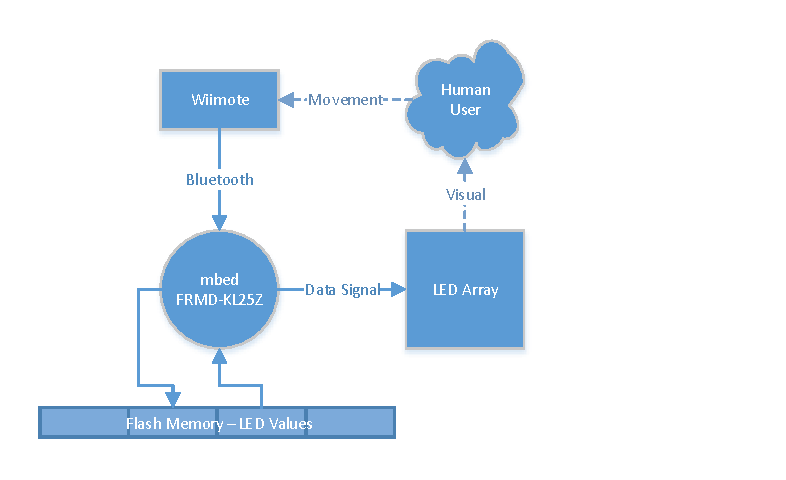
\includegraphics[trim=1cm 0cm 4cm 0cm, width=\linewidth]{dataflow.pdf}
    \caption{Data Flow and Project Structure}
\end{marginfigure}
\subsection{LED Array Hardware}
Our plan originally assumed that the individually-addressable LED strips
available from the lab were
the 30 LEDs per meter variety, but it turns out that they have twice the LED
density at 60 LEDs per meter. This was problematic--a larger screen helps
reduce the effects of error in determining Wiimote pointing direction making
for a better user experience, and a
screen built with 60 LEDs per meter strips is a quarter the size of the original
if the 30x30 resolution is maintained. 
%\begin{marginfigure}[-2\baselineskip]
        %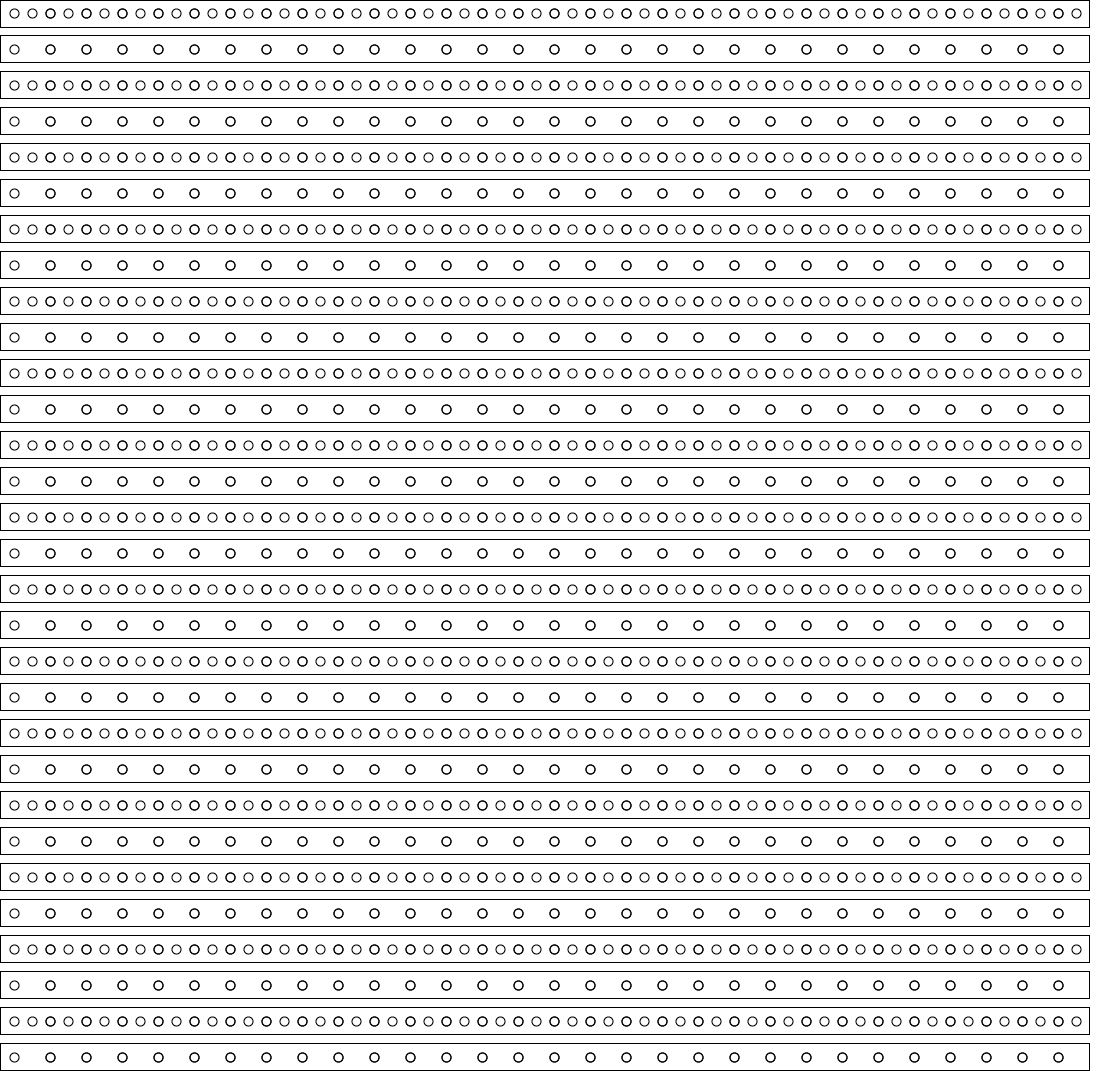
\includegraphics[width=\linewidth]{array.png}
        %\caption{Layout of LED strips. Alternates between 60 LED per meter
        %strip and 30 LED per meter strip.}
%\end{marginfigure}
Additionally, we ended up with 15
meters of 60 LEDs per meter strip from the lab, and 15 meters of 30 LEDs per
meter strip that we already had. 
We modified our design so that the screen
would still be a square meter by using the 60 LEDs per meter strips as 30 LEDs
per meter strips by only turning on every other LED, which so far seems to be
a viable solution.
\begin{figure}
    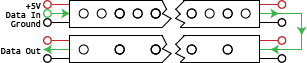
\includegraphics{Wiring_Diagram.png}
    \caption{LED Strip Wiring. A 1 meter length of 30 LED per meter strip is
    attached to the end of a 1 meter length of 60 LED per meter strip. This
lets us connect fifteen total strips of 90 LEDs to the microcontroller,
instead of thirty strips. The software needs to have some model of the
physical arrangement of LEDs, so that it can properly address each LED.}
\end{figure}

\subsection{Microcontroller Software}
To control the LEDs, we are using the Multi\_WS2811 library\sidenote{This
library is by Ned Konz for the FRDM-KL25Z, and is made available to us under
the Apache License.} This library can control up to 16 strips of LEDs in
parallel using 3-phase DMA transfers\sidenote{The number of parallel LED
strips is limited to at most the number of pins on a single GPIO port for the
microcontroller.}. However, as initially written, this library cannot support
the number of LEDs per strip that we need it to in the available amount of RAM
on the device. At 80 LEDs per strip, the library takes approximately 98\% of
the RAM on the microcontroller. To remedy this, we moved a large run-time
constant array from RAM to Flash\sidenote{The downside to this approach is that we must now hardcode all values of the array instead of using \texttt{memset}, which requires more work on the part of the programmer, but does not affect functionality of the library.}, which reduced RAM usage to 57\% at 90 LEDs per strip.

\subsection{Power}
Although datasheets for the specific model of LED strips we have were not
available, a common upper-bound\sidenote{This occurs when the LED is set to
full brightness white. Average consumption is much lower} for WS2812b-based 
LEDs is 60 mA per LED\sidenote{Burgess, Phillip.``Powering NeoPixels.''
    \textit{Adafruit}. 30 Aug 2013. Web.
    \url{https://learn.adafruit.com/adafruit-
    neopixel-uberguide/power}}. Average-case current draw is typically around
    20 mA. For an array of 900 LEDs, this comes out to a total current draw
    from 18 A to 54 A at 5 volts. To make the system as safe as possible, the
    LED array hardware must be designed to distribute this current evenly and
    handle peak usage without catching fire. ``Peak usage'' can be drastically
    lowered by limiting the LED brightness in software, and designing the
    system behavior to reduce the frequency of high current draw
    states\sidenote{This can be done in a variety of ways. One example is
        having the default ``blank'' screen non-white. If the LEDs are off
        instead of white, then initally the array will use very little power,
    instead of the maximum possible.}
\section{Future}

For the remainder of the project, we need to finish assembling the LED
hardware, finalize and test reading from and/or writing to the Wiimote and
LEDs. Additionally, we need to write the software that updates LED color based
on Wiimote position, and we need to determine where on the screen the Wiimote
is pointing within a reasonable degree of accuracy.


\end{document}
